%%%%%%%%%%%%%%%%%%%%%%%%%%%%%%%%%%%%%%%%%
% Beamer Presentation
% LaTeX Template
% Version 1.0 (10/11/12)
%
% This template has been downloaded from:
% http://www.LaTeXTemplates.com
%
% License:
% CC BY-NC-SA 3.0 (http://creativecommons.org/licenses/by-nc-sa/3.0/)
%
%%%%%%%%%%%%%%%%%%%%%%%%%%%%%%%%%%%%%%%%%

%----------------------------------------------------------------------------------------
%	PACKAGES AND THEMES
%----------------------------------------------------------------------------------------

\documentclass[aspectratio=169]{beamer}
%%\documentclass{beamer}
\mode<presentation> {

% The Beamer class comes with a number of default slide themes
% which change the colors and layouts of slides. Below this is a list
% of all the themes, uncomment each in turn to see what they look like.

%\usetheme{default}
%\usetheme{AnnArbor}
%\usetheme{Antibes}
%\usetheme{Bergen}
%\usetheme{Berkeley}
%\usetheme{Berlin}
%\usetheme{Boadilla}
%\usetheme{CambridgeUS}
%\usetheme{Copenhagen}
%\usetheme{Darmstadt}
%\usetheme{Dresden}
%\usetheme{Frankfurt}
%\usetheme{Goettingen}
%\usetheme{Hannover}
%\usetheme{Ilmenau}
%\usetheme{JuanLesPins}
%\usetheme{Luebeck}
\usetheme{Madrid}
%\usetheme{Malmoe}
%\usetheme{Marburg}
%\usetheme{Montpellier}
%\usetheme{PaloAlto}
%\usetheme{Pittsburgh}
%\usetheme{Rochester}
%\usetheme{Singapore}
%\usetheme{Szeged}
%\usetheme{Warsaw}

% As well as themes, the Beamer class has a number of color themes
% for any slide theme. Uncomment each of these in turn to see how it
% changes the colors of your current slide theme.

%\usecolortheme{albatross}
%\usecolortheme{beaver}
%\usecolortheme{beetle}
%\usecolortheme{crane}
%\usecolortheme{dolphin}
%\usecolortheme{dove}
%\usecolortheme{fly}
%\usecolortheme{lily}
%\usecolortheme{orchid}
%\usecolortheme{rose}
%\usecolortheme{seagull}
%\usecolortheme{seahorse}
%\usecolortheme{whale}
%\usecolortheme{wolverine}

%\setbeamertemplate{footline} % To remove the footer line in all slides uncomment this line
%\setbeamertemplate{footline}[page number] % To replace the footer line in all slides with a simple slide count uncomment this line

%\setbeamertemplate{navigation symbols}{} % To remove the navigation symbols from the bottom of all slides uncomment this line
}
%%\documentclass[mathserif,hyperref={pdfpagemode=FullScreen}]{beamer}
%%% \documentclass[handout]{beamer}
%%% \usetheme{Dresden}
%%\usetheme{340}
%%\beamertemplatetransparentcovereddynamic
%%\usepackage[latin1]{inputenc}
%%\usepackage{pgf}


\usepackage{amsmath,amsfonts,amssymb}
\usepackage{xspace}
\usepackage{algorithm}
\usepackage{algorithmic}
\usepackage{xcolor}
\usepackage{graphicx} % Allows including images
\usepackage{booktabs} % Allows the use of \toprule, \midrule and \bottomrule in tables
%%\usepackage{xspace}

\usepackage{braket}
\usepackage{multirow}
\usepackage{todonotes}


\usepackage{appendixnumberbeamer}


%%\usepackage{enumitem}


\newcommand{\heteroprio}{{HeteroPrio}\xspace}
\newcommand{\heteroprioD}{{HeteroPrioDep}\xspace}


%%\usepackage{tcolorbox}
\usepackage{tikz}
\usetikzlibrary{matrix, decorations, patterns, positioning, shapes, calc, intersections, arrows, fit}


\usetikzlibrary{patterns}
\usetikzlibrary{fit,calc,positioning,decorations.pathreplacing,matrix}

\graphicspath{{./diagrams/}{./plots/}}

%%\tikzset{xtick/.style={inner xsep=0pt, inner ysep=3pt, minimum
%%		size=0pt, draw, label=below:#1},%
%%	comm/.style args={#1start#2length#3color#4}{rounded corners=1mm, draw, inner
%%		sep=0pt, fill=#4, label=center:#1, fit={(#2,0.75)
%%			(#2+#3,1.5)}},%
%%	comp/.style args={#1start#2length#3color#4}{rounded corners=1mm, draw, inner
%%		sep=0pt, fill=#4, label=center:#1, fit={(#2,0)
%%			(#2+#3,0.75)}},%
%%}
%%
%%\newcommand{\schedule}[3]{
%%	\draw[->] (-0.2, 0) -- (#1, 0) node[below] {$t$};
%%	\draw (0, 0) -- (0, 1.5);
%%	\node at (-0.8, 0.75)[rotate=90] {#2};
%%	\draw[dashed,gray] (0, 0.75) -- (#1, 0.75);
%%	\foreach \t in {0,#3} {
%%		\node[xtick=\t] at (\t, 0){};
%%	}
%%}
%%\newcommand{\task}[6][0]{
%%	\node[comm=#2 start #3 length #4 color #6]{};
%%	\node[comp=#2 start #3+#4+#1 length #5 color #6]{}; 
%%}


\newcommand\addvmargin[1]{
	\node[fit=(current bounding box),inner ysep=#1,inner xsep=0]{};
}

\newcommand{\tensor}[1]{{\cal\textbf{#1}\xspace}}
\newcommand{\ttrain}{{\it Tensor-Train}\xspace}

\newcommand{\hfirst}{{\it LSR}\xspace}
\newcommand{\hsecond}{{\it SLSB}\xspace}
\newcommand{\hthird}{{\it LSB}\xspace}
\newcommand{\otta}{{\it STTA}\xspace}


\newcommand{\credit}[1]{\vspace*{-0.2cm}\par\hfill {\footnotesize Source:~\itshape#1}}

%%\newcommand{\tensorcolor}{patternblue}
\newcommand{\tensorcolor}{cyan}

%% Colors from https://latexcolor.com/
\definecolor{pastelviolet}{rgb}{0.8, 0.6, 0.79}
\definecolor{babyblueeyes}{rgb}{0.63, 0.79, 0.95}
\definecolor{pastelyellow}{rgb}{0.99, 0.99, 0.59}
%%\definecolor{pastelgreen}{rgb}{0.47, 0.87, 0.47}
\definecolor{pastelgreen}{rgb}{0, 1, 0}
\definecolor{pastelred}{rgb}{1.0, 0.41, 0.38}
\colorlet{patternblue}{blue!60}




\definecolor{forestgreen}{rgb}{0.13, 0.55, 0.13}
\definecolor{greenhtml}{rgb}{0.0, 0.5, 0.0}
\definecolor{cyannew}{rgb}{0.0, 1.0, 1.0}


\newcommand{\mycolora}{green}
\newcommand{\mycolorb}{blue}
\newcommand{\mycolorc}{cyan}
\newcommand{\mycolord}{violet}
\newcommand{\mycolore}{orange}
\newcommand{\mycolorf}{forestgreen}


\newcommand{\mysymbola}{\textcolor{\mycolora}{$\blacksquare$}}
\newcommand{\mysymbolb}{\textcolor{\mycolorb}{$\blacksquare$}}
\newcommand{\mysymbolc}{\textcolor{\mycolorc}{$\blacksquare$}}
\newcommand{\mysymbold}{\textcolor{\mycolord}{$\blacksquare$}}
\newcommand{\mysymbole}{\textcolor{\mycolore}{$\blacksquare$}}
\newcommand{\mysymbolf}{\textcolor{\mycolorf}{$\blacksquare$}}


\newcommand{\mybullet}{\textcolor{blue}{$\quad\bullet$}\xspace}

%%\newcommand{\mysymbola}{\mycolorb}
%%\newcommand{\mysymbola}{\mycolorc}
%%\newcommand{\mysymbola}{\mycolord}
%%\newcommand{\mysymbola}{\mycolore}
%%\newcommand{\mysymbola}{\mycolorf}



%----------------------------------------------------------------------------------------
%	TITLE PAGE
%----------------------------------------------------------------------------------------

\title[Scalable Tensor Algorithms]{Scalable Tensor Algorithms for Modern Computing Systems} % The short title appears at the bottom of every slide, the full title is only on the title page

\author[Suraj {\sc Kumar}]{Suraj {\sc Kumar}} % Your name
%%\institute[UCLA] % Your institution as it will appear on the bottom of every slide, may be shorthand to save space\institute[Inria Paris] % Your institution as it will appear on the bottom of every slide, may be shorthand to save space
%%{
%%	Alpines team, Inria Paris, France\\ % Your institution for the title page
%%	\medskip
%%	\textit{Suraj.kumar@inria.fr} % Your email address
%%}
%%{
%%University of California \\ % Your institution for the title page
%%\medskip
%%\textit{john@smith.com} % Your email address
%%}

\institute[ROMA Applicant]{Inria ROMA Applicant}
%%%%\institute[Inria Paris] % Your institution as it will appear on the bottom of every slide, may be shorthand to save space
%%%%{
%%%%	Alpines team, Inria Paris, France\\ % Your institution for the title page
%%%%	\medskip
%%%%	\textit{Suraj.kumar@inria.fr} % Your email address
%%%%}
\date{\today} % Date, can be changed to a custom date



\makeatletter
\AtBeginPart{%
	\beamer@tocsectionnumber=0\relax
	\setcounter{section}{0}
%%	\frame{\partpage}%
}
\makeatother

\begin{document}

\begin{frame}
\titlepage % Print the title page as the first slide
\end{frame}






\appendix


\begin{frame}
\Huge{\centerline{Backup Slides}}
\end{frame}

% And your backup slides here
\begin{frame}{Our Performance Bound}
\begin{columns}
	\begin{column}[c]{.475\linewidth}
		\begin{block}{\centering {\scriptsize Task Graph}}
			\only<1-3> {\centering \includegraphics[scale=0.25]{boundsDiagram/taskgraph}}
			%\only<2-3> {\centering 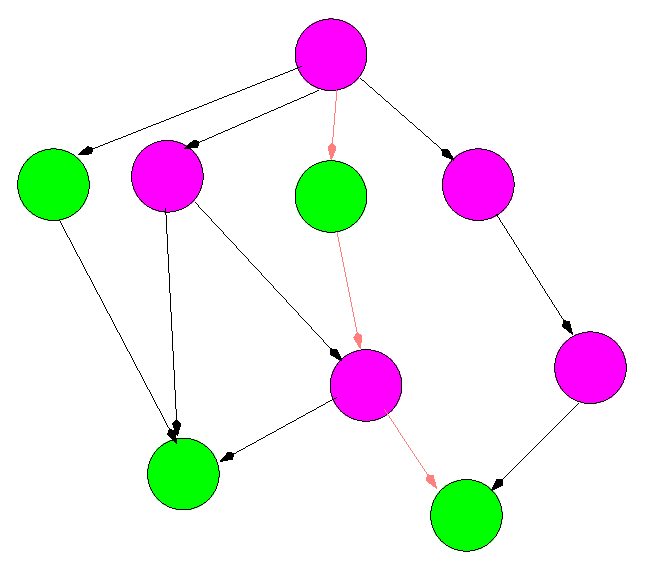
\includegraphics[scale=0.25]{boundsDiagram/taskgraphPath}}
		\end{block}
	\end{column}\hfill
	\begin{column}[c]{.475\linewidth}
		\begin{block}{\centering {\scriptsize \only<1> {No} \only<2-3> {Some} 
					Dependencies}}
			\only<1> {\centering \includegraphics[scale=0.25]{boundsDiagram/taskgraphNoDep}}
			\only<2-3> {\centering \includegraphics[scale=0.25]{boundsDiagram/taskgraphOnePath}}
		\end{block}
	\end{column}
\end{columns}
\begin{block}{\centering {\scriptsize Minimum execution time (minimize \textit{l})}}
	\begin{columns}
		\begin{column}[c]{.5\linewidth}
			\centering \includegraphics[scale=0.45]{boundsDiagram/schedule}   
		\end{column}
		\begin{column}[c]{.5\linewidth}
			\only<2-3>
			{
				\begin{itemize}
					\item[$\star$]{\scriptsize If any path in the graph is larger than \textit{l}}
					\only<3>{
						\begin{itemize}
							\item {\scriptsize add this path as a constraint and repeat the procedure}
						\end{itemize}
					}
				\end{itemize}
			}
			
		\end{column}  
	\end{columns}
\end{block}

\end{frame}

\begin{frame}{Roofline model with Dependencies}
%%\begin{columns}
%%	\begin{column}{0.45\linewidth}
%%	\end{column}
%%\end{columns}
\vspace*{-0.35cm}
\begin{center}
\begin{minipage}{0.425\linewidth}
	\begin{block}{Our bound}
\centering \includegraphics[scale=0.285]{boundsDiagram/taskgraphOnePath}
	\end{block}
\end{minipage}$\qquad$
\begin{minipage}{0.425\linewidth}
	\begin{block}{Roofline Model}
			\includegraphics[scale=0.14]{./diagrams/Example_of_a_Roofline_model.png}
	\end{block}
\end{minipage}
\end{center}
%\begin{columns}
%	\begin{column}[c]{.5\linewidth}
%		\begin{block}{\centering {\scriptsize DAG}}
%			\only<1-3> {\centering \includegraphics[scale=0.25]{boundsDiagram/taskgraph}}
%			%\only<2-3> {\centering 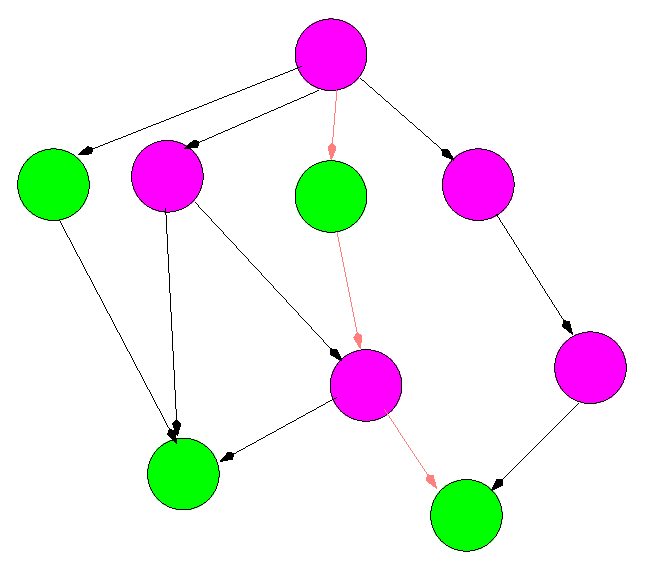
\includegraphics[scale=0.25]{boundsDiagram/taskgraphPath}}
%		\end{block}
%	\end{column}
	
%%	\begin{column}[c]{.5\linewidth}
%%		\begin{block}{\centering {\scriptsize \only<1> {No} \only<2-3> {Some} 
%%					Dependencies}}
%%			\only<1> {\centering \includegraphics[scale=0.25]{boundsDiagram/taskgraphNoDep}}
%%			\only<2-3> {\centering \includegraphics[scale=0.25]{boundsDiagram/taskgraphOnePath}}
%%		\end{block}
%%	\end{column}
%%\end{columns}
\begin{block}{\centering {\scriptsize Minimum execution time (minimize \textit{l})}}
	\begin{columns}
		\begin{column}[c]{.5\linewidth}
			\centering \includegraphics[scale=0.45]{boundsDiagram/schedule}   
		\end{column}
		\begin{column}[c]{.5\linewidth}
			\begin{itemize}
					\item[$\star$]{\scriptsize If any path in DAG is larger than \textit{l}}
						\begin{itemize}
							\item {\scriptsize add this path with data transfer cost as a constraint and repeat the procedure}
						\end{itemize}
				\end{itemize}			
		\end{column}  
	\end{columns}
\end{block}
\vspace*{-0.25cm}
\begin{itemize}
	\item Take minimum of both values as the lower bound of the application
\end{itemize}
\end{frame}


\begin{frame}{Unfolding matrices of a tensor}

{\small
\vspace*{-0.15cm}\begin{block}{}
	\begin{center}
		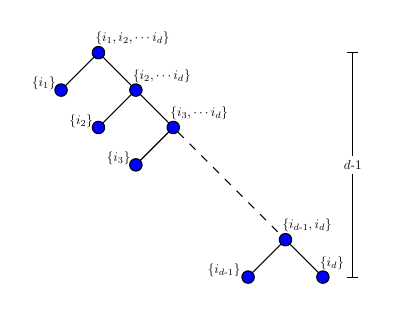
\begin{tikzpicture}[scale=0.475, every node/.style={transform shape}]
%%\draw[fill=cyan] (0,0) circle (0.8cm);
%%		\node [draw,circle]{r};
%%		\tikzstyle{task}=[circle, draw, minimum size=10mm]
%%		\node (d) at (0,0)[task, fill=babyblueeyes] {$D$};
%%		\node (e) at (2.5,0)[task, fill=pastelviolet] {$E$};
%%		\draw[thick, ->] (d.east) -- (e);
%%		
%%		\node (a) at (0,2)[task, fill=pastelyellow] {$A$};
%%		\node (b) at (2.5,2.75)[task, fill=pastelgreen] {$B$};
%%		\node (c) at (2.5,1.25)[task, fill=pastelred] {$C$};
%%		
%%		\draw[thick, ->] (a.east) -- (b);
%%		\draw[thick, ->] (a.east) -- (c);
\tikzstyle{taskc}=[circle, draw=black, minimum size=2mm, fill=blue]
\tikzstyle{taskr}=[draw=none, minimum height=2mm, minimum width=5mm, anchor=south west, fill=none, text=black]
%%
\node (t01) at (0,0) [taskc]{};
\node (t11) at (-1,-1) [taskc] {};
\node (t12) at (1, -1) [taskc] {};
\node (t21) at (0, -2) [taskc] {};
\node (t22) at (2, -2) [taskc] {};
\node (t31) at (1,-3) [taskc] {};
\node (t52) at (5, -5) [taskc] {};
\node (t61) at (4, -6) [taskc] {};
\node (t62) at (6, -6) [taskc] {};

\draw (t01) -- (t11);
\draw (t01) -- (t12);
\draw (t12) -- (t21);
\draw (t12) -- (t22);
\draw (t22) -- (t31);
\draw [dashed] (t22) -- (t52);
\draw (t52) -- (t61);
\draw (t52) -- (t62);

\draw (6.8, -6) -- (6.8, -3.25);
\draw (6.8, -2.75) -- (6.8, 0);

\draw (6.65, -6) -- (6.95, -6);
\draw (6.65, -0) -- (6.95, 0);
\node at (6.8, -3) {$d\text{-}1$};

\node [above left=0mm and 2mm of t01.mid, taskr](l01) {$\{i_1,i_2,\cdots i_d\}$};
\node [below left=2mm and 9mm of t11.mid, taskr](l11) {$\{i_1\}$};
\node [above left=0mm and 2mm of t12.mid, taskr](l12) {$\{i_2,\cdots i_d\}$};
\node [below left=2mm and 9mm of t21.mid, taskr](l21) {$\{i_2\}$};
\node [above left=0mm and 2mm of t22.mid, taskr](l22) {$\{i_3,\cdots i_d\}$};
\node [below left=2mm and 9mm of t31.mid, taskr](l31) {$\{i_3\}$};

\node [above left=0mm and 2mm of t52.mid, taskr](l52) {$\{i_{d\text{-}1}, i_d\}$};
\node [below left=2mm and 12mm of t61.mid, taskr](l61) {$\{i_{d\text{-}1}\}$};
\node [above left=0mm and 2mm of t62.mid, taskr](l62) {$\{i_d\}$};

\path (-0.1, -6.4) -- (2.5, -6.4); 
\end{tikzpicture}$\qquad$
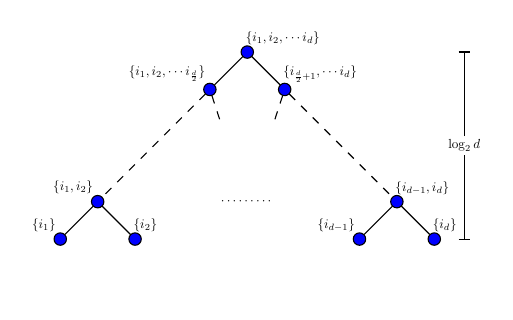
\begin{tikzpicture}[scale=0.475, every node/.style={transform shape}]

\tikzstyle{taskc}=[circle, draw=black, minimum size=2mm, fill=blue]
%%	\tikzstyle{taskr}=[draw=none, minimum height=2mm, minimum width=5mm, anchor=south west, fill=none, text=black]


\node (t01) at (0,0) [taskc]{};
\node (t11) at (-1,-1) [taskc] {};
\node (t12) at (1, -1) [taskc] {};

\node (tinter1) at (-0.5,-2) [taskc, draw=none, fill=none] {};
\node (tinter2) at (0.5,-2) [taskc, draw=none, fill=none] {};

\node (t41) at (-4,-4) [taskc] {};
\node (t42) at (4,-4) [taskc] {};
\node (t51) at (-5,-5) [taskc] {};
\node (t52) at (-3,-5) [taskc] {};
\node (t53) at (3,-5) [taskc] {};
\node (t54) at (5,-5) [taskc] {};


\draw (t01) -- (t11);
\draw (t01) -- (t12);

\draw [dashed] (t11) -- (tinter1.west);
\draw [dashed] (t12) -- (tinter2.east);

\draw [dashed] (t11) -- (t41);
\draw [dashed] (t12) -- (t42);

\path (t41) -- (t42) node [midway] {$\cdots\cdots\cdots$};

\draw (t41) -- (t51);
\draw (t41) -- (t52);

\draw (t42) -- (t53);
\draw (t42) -- (t54);


\draw (5.8, -5) -- (5.8, -2.75);
\draw (5.8, -2.25) -- (5.8, 0);

\draw (5.65, -5) -- (5.95, -5);
\draw (5.65, 0) -- (5.95, 0);
\node at (5.8, -2.5) {$\log_2 d$};

\node [above right] at (t01.160) {$\{i_1,i_2,\cdots i_d\}$};	

\node [above left] at (t11.mid) {$\{i_1,i_2,\cdots i_\frac{d}{2}\}$};	
\node [above right] at (t12.160) {$\{i_{\frac{d}{2}+1},\cdots i_d\}$};

\node [above left] at (t41.mid) {$\{i_1,i_2\}$};
\node [above right] at (t42.160) {$\{i_{d-1}, i_d\}$};

\node [above left] at (t51.mid) {$\{i_1\}$};
\node [above right] at (t52.160) {$\{i_2\}$};

\node [above left] at (t53.mid) {$\{i_{d-1}\}$};
\node [above right] at (t54.160) {$\{i_d\}$};


\path (-0.1, -6.4) -- (2.5, -6.4); 
%%		\path (-6.5, 0) -- (0,0);
\end{tikzpicture}
\end{center}
\end{block}
%%\begin{block}{$k$-th unfolding matrix}
	$k$-th unfolding matrix of tensor $\tensor{A}$ is defined as, $ A_k = [A_k(i_1, i_2,\cdots, i_k; i_{k+1},\cdots ,i_d)]$
	
	\begin{itemize}
		\item Size of $A_k$ is $(\prod_{l=1}^{k}n_l)\times(\prod_{l=k+1}^{d}n_l)$
		\item $r_k$ = rank($A_k$)
		\item Each node works with an unfolding matrix 
	\end{itemize}
%%\end{block}
\vspace*{-0.15cm}
\begin{block}{}
Theorem: Our parallel algorithm produces a Tensor Train representation with ranks not higher than $r_k$.
\end{block}
}\end{frame}


\begin{frame}{Communication Computation Overlap}
\begin{columns}
	\begin{column}{0.55\textwidth}
		\begin{center}
			\begin{tabular}{|c|c|c|}
				\hline
				Task & Data Transfer Time & Computation Time\\ \hline
				\textcolor{purple}{A} & 5 & 3 \\
				\textcolor{teal}{B} & 2 & 4 \\ \hline
			\end{tabular}
		\end{center}
		\noindent Problem: Given a set of tasks in what order we transfer them from $M$ to $C$ such that the makespan is minimal?
	\end{column}
	\begin{column}{0.35\textwidth}
		
		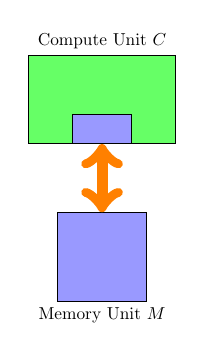
\begin{tikzpicture}[scale=0.625, every node/.style={transform shape}]
		\tikzstyle{taskmemory}=[draw=black, minimum height=18mm, minimum width=18mm, fill=blue!40, text=black]
		\tikzstyle{taskcompute}=[draw=black, minimum height=18mm, minimum width=30mm, fill=green!60, text=black]
		
		\node (tm) at (0,0) [taskmemory] {}; 
		\node (tc) at (0,32mm) [taskcompute] {};
		
		\draw [<->, line width=4, orange] (tm) -- (tc);
		
		\node [below] at (tm.south) {Memory Unit $M$};
		\node [above] at (tc.north) {Compute Unit $C$};
		
		\node [taskmemory, minimum height=6mm, minimum width=12mm, anchor=south] at (tc.south) {}; 
		\end{tikzpicture}
		
		%%\begin{tikzpicture}[scale=0.625, every node/.style={transform shape}]
		%%\tikzstyle{taskr}=[draw=black, minimum height=1mm, minimum width=12mm, anchor=south west, fill=pastelgreen, text=black]
		%%			\node (t01) at (0,0) [taskr]{};
		%%\end{tikzpicture}
		%%\begin{tikzpicture}
		%%\pgfmathsetmacro{\cubex}{5}
		%%\pgfmathsetmacro{\cubey}{1}
		%%\pgfmathsetmacro{\cubez}{3}
		%%\draw[red,fill=yellow] (0,0,0) -- ++(-\cubex,0,0) -- ++(0,-\cubey,0) -- ++(\cubex,0,0) -- cycle;
		%%\draw[red,fill=yellow] (0,0,0) -- ++(0,0,-\cubez) -- ++(0,-\cubey,0) -- ++(0,0,\cubez) -- cycle;
		%%\draw[red,fill=yellow] (0,0,0) -- ++(-\cubex,0,0) -- ++(0,0,-\cubez) -- ++(\cubex,0,0) -- cycle;
		%%\end{tikzpicture}
		%%	\includegraphics[scale=0.02]{./tmp/memorytoComputeUnit.jpg}
	\end{column}
\end{columns}

\vspace*{-0.15cm}
\begin{exampleblock}{Possible schedules}
	\begin{center}
		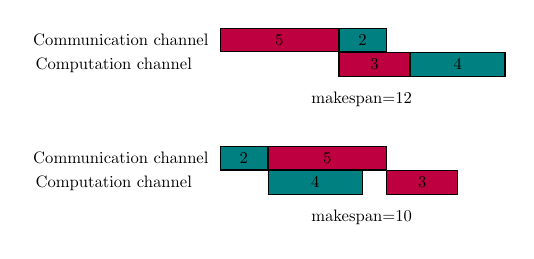
\begin{tikzpicture}[scale=0.6, every node/.style={transform shape}]
		\tikzstyle{taskA}=[draw=black, minimum height=5mm, fill=purple, text=black]
		\tikzstyle{taskB}=[draw=black, minimum height=5mm, fill=teal, text=black]
		
		\node (tcommA) at (0,0) [taskA, minimum width=25mm, anchor=south west] {$5$};
		\node (tcompA) at (tcommA.south east) [taskA, minimum width=15mm, anchor=north west] {$3$};
		
		\node (tcommB) at (tcommA.south east) [taskB, minimum width=10mm, anchor=south west] {$2$};
		\node (tcompB) at (tcompA.north east) [taskB, minimum width=20mm, anchor=north west] {$4$};
		
		\node at (tcommA.west) [left] {Communication channel$\ $};
		\node at (tcommA.south west) [below left] {Computation channel $\quad$};
		
		\node at (3,-1) {makespan=12};
		
		
		\node (tcommB) at (0,-2.5) [taskB, minimum width=10mm, anchor=south west] {$2$};
		\node (tcompB) at (tcommB.south east) [taskB, minimum width=20mm, anchor=north west] {$4$};
		
		\node (tcommA) at (tcommB.south east) [taskA, minimum width=25mm, anchor=south west] {$5$};
		\node (tcompA) at (tcommA.south east) [taskA, minimum width=15mm, anchor=north west] {$3$};
		
		\node at (tcommB.west) [left] {Communication channel$\ $};
		\node at (tcommB.south west) [below left] {Computation channel $\quad$};
		
		\node at (3,-3.5) {makespan=10};
		
		\end{tikzpicture}
	\end{center}
\end{exampleblock}
%%\includegraphics[scale=0.02]{./tmp/taskOptimalOrderExample.jpg}

%%\begin{block}{Problem $DT$ }
%%	\begin{itemize}
%%		\item A set of tasks $ST=\{T_1, \cdots, T_n\}$ is scheduled on a processing unit $P$ with
%%		memory unit $M$ of capacity $C$
%%		\item Input data for tasks of $ST$
%%		reside on another memory unit
%%		\item Tasks do not produce output data
%%		\item Tasks do not require intermediate memory
%%		\item A tasks uses an amount of memory in $M$ from the
%%		start of its communication to the end of its computation
%%	\end{itemize}
%%	\noindent Given $L$, is there a feasible schedule $S$ for $ST$ such that
%%	makespan of $S$, $\mu(S) \le L$?
%%\end{block}
\end{frame}

\begin{frame}[fragile]{Order of Data Transfers}
\begin{itemize}
\item Compute intensive task: Computation time $\ge$ Data transfer time
\item Communication intensive task: Computation time $<$ Data transfer time
\end{itemize}
\begin{block}{Optimal Algorithm: When memory capacity of the compute unit is not a concern}
\begin{itemize}
	\item First sort compute intensive tasks in increasing order of their data transfer time
	\item Then sort the communication intensive tasks in decreasing order of their computation time 
\end{itemize}
\end{block}

\newcommand{\threepart}{\textsc{3Par}\xspace}
\begin{block}{Memory capacity is limited}
\begin{itemize}
	\item Proved that the problem is NP-Complete
	%%\begin{itemize}
	%%	\item Reduced \threepart problem to this problem
	%%\end{itemize} 
	\item Proposed static and dynamic based approaches and evaluated them on traces of molecular simulations
	\begin{itemize}
		\item Static approaches: order is computed  in advance
		\item Dynamic approaches: next task is chosen based on the heuristic
		\item Combination of both: start with static order and switch to dynamic based on available memory
	\end{itemize}
	%%\item Implemented static approaches also in Tensor Algebra for Manybody Methods (TAMM) library
\end{itemize}

%%\tikzset{xtick/.style={inner xsep=0pt, inner ysep=3pt, minimum size=0pt, draw},%
%%task/.style args={#1start#2length#3res#4color#5}{rounded corners, draw, inner sep=0pt, fill=#5, label=center:#1, fit={(#2,#4*0.75) (#2+#3,#4*0.75+0.75)}},%
%%vert/.style={inner sep=1pt, fill=black, circle, draw, label=#1}
%%}
%%\newcommand{\scheduleNoName}[1]{
%%\draw[->] (-0.4, 0) -- (#1, 0) node[below] {$t$};
%%\draw (0, 0) -- (0, 1.5) node[pos=0.25, left] {Comp.}
%%node[pos=0.75, left] {Comm.};
%%\draw[dashed,gray] (0, 0.75) -- (#1, 0.75);
%%}
%%
%%
%%\begin{center}
%%\begin{tikzpicture}[yscale=0.7, thick, xscale=0.6]
%%\scheduleNoName{12.5}
%%\node[task=$A_{1,1}$ start 0 length 1 res 1 color cyan]{};
%%\node[task=$A_{1,2}$ start 1 length 1 res 1 color blue!40!white]{};
%%\node[task=$A_{1,3}$ start 2 length 1 res 1 color blue!70!white]{};
%%\node[task=$K_0$ start 0 length 3 res 0 color gray!40!white]{};
%%\node[task=$K_1$ start 3 length 6 res 1 color green]{}; 
%%\node[task=$A_{1,1}$ start 3 length 1.8 res 0 color cyan]{};
%%\node[task=$A_{1,2}$ start 4.8 length 2.3 res 0 color blue!40!white]{};
%%\node[task=$A_{1,3}$ start 7.1 length 1.9 res 0 color blue!70!white]{};
%%\node[task=$A_{2,1}$ start 9 length 1 res 1 color cyan]{};
%%\node[task=$A_{2,2}$ start 10 length 1 res 1 color blue!40!white]{};
%%\node[task=$A_{2,3}$ start 11 length 1 res 1 color blue!70!white]{};
%%\node[task=$K_1$ start 9 length 3 res 0 color green]{};
%%%%	\draw[<->,thin] (0, -0.2) -- node[below]{$3$} (3, -0.2) ;
%%%%	\draw[<->,thin] (9, -0.2) -- node[below]{$3$} (12, -0.2) ;
%%%%	\draw[<->,thin] (3, -0.2) -- node[below]{$b'$} (9, -0.2) ;
%%\draw[<->,thin] (0, -0.2) -- (3, -0.2) ;
%%\draw[<->,thin] (9, -0.2) -- (12, -0.2) ;
%%\draw[<->,thin] (3, -0.2) -- (9, -0.2) ;
%%\end{tikzpicture}
%%\end{center}
\end{block}
\end{frame}


%%\begin{frame}{NP-Completeness Structure}
%%content...
%%\end{frame}
\begin{frame}{Performance evaluation on Summit supercomputer}


\begin{itemize}
\item Implemented static approaches in Tensor Algebra for Manybody Methods (TAMM) library
\item CCSD application, Ubiqtin molecule, cc-pVDZ (737 basis functions, 220 nodes), aug-cc-pVDZ (1243 basis functions, 256 nodes)
\end{itemize}
\begin{columns}
\begin{column}{0.56\linewidth}
\begin{center}
	\includegraphics[scale=0.13]{./diagrams/Summit_Node.jpg}
	
	\vspace*{-0.25cm}{\tiny \hspace*{2cm} Fig source: \url{https://www.olcf.ornl.gov}}
\end{center}
\end{column}
\begin{column}{0.45\linewidth}
\includegraphics[scale=0.5]{./diagrams/tamm-performance.eps}
\end{column}
\end{columns}
\end{frame}







\begin{frame}{Architecture Aware Algorithms}
\begin{center}
	\begin{minipage}{0.45\columnwidth}
			\includegraphics[scale=0.25]{./diagrams/VoltaTensorCore.png}
	\end{minipage}
	\begin{minipage}{0.45\columnwidth}
		\includegraphics[scale=0.25]{./diagrams/A100_TensorCore_FP64.jpg}
	\end{minipage}
\end{center}
\begin{itemize}
	\item Recent Nvidia GPUs have tensor cores to accelerate AI computations
	\item Most linear algebra computations do not take advantages of these units
	\item Design algorithms which take architecture details into account
\end{itemize}
Fig source: \url{www.nvidia.com}
\end{frame}


\begin{frame}{Order of separation of dimensions in tensor train algorithms}

{\small\vspace*{-0.25cm}
	\begin{itemize}
		\item  Determine the order of separation of dimensions
	\end{itemize}
	\begin{minipage}{0.425\linewidth}
		\begin{block}{Sequential algorithm}
			\begin{center}
				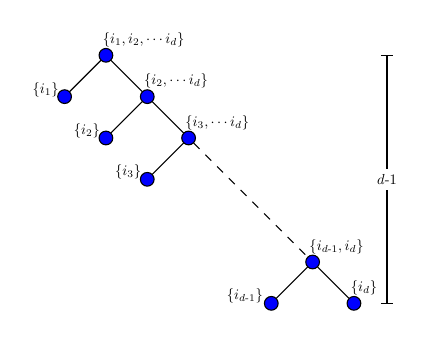
\begin{tikzpicture}[scale=0.525, every node/.style={transform shape}]
				\tikzstyle{taskc}=[circle, draw=black, minimum size=2mm, fill=blue]
				\tikzstyle{taskr}=[draw=none, minimum height=2mm, minimum width=5mm, anchor=south west, fill=none, text=black]
				%%
				\node (t01) at (0,0) [taskc]{};
				\node (t11) at (-1,-1) [taskc] {};
				\node (t12) at (1, -1) [taskc] {};
				\node (t21) at (0, -2) [taskc] {};
				\node (t22) at (2, -2) [taskc] {};
				\node (t31) at (1,-3) [taskc] {};
				\node (t52) at (5, -5) [taskc] {};
				\node (t61) at (4, -6) [taskc] {};
				\node (t62) at (6, -6) [taskc] {};
				
				\draw (t01) -- (t11);
				\draw (t01) -- (t12);
				\draw (t12) -- (t21);
				\draw (t12) -- (t22);
				\draw (t22) -- (t31);
				\draw [dashed] (t22) -- (t52);
				\draw (t52) -- (t61);
				\draw (t52) -- (t62);
				
				\draw (6.8, -6) -- (6.8, -3.25);
				\draw (6.8, -2.75) -- (6.8, 0);
				
				\draw (6.65, -6) -- (6.95, -6);
				\draw (6.65, -0) -- (6.95, 0);
				\node at (6.8, -3) {$d\text{-}1$};
				
				\node [above left=0mm and 2mm of t01.mid, taskr](l01) {$\{i_1,i_2,\cdots i_d\}$};
				\node [below left=2mm and 9mm of t11.mid, taskr](l11) {$\{i_1\}$};
				\node [above left=0mm and 2mm of t12.mid, taskr](l12) {$\{i_2,\cdots i_d\}$};
				\node [below left=2mm and 9mm of t21.mid, taskr](l21) {$\{i_2\}$};
				\node [above left=0mm and 2mm of t22.mid, taskr](l22) {$\{i_3,\cdots i_d\}$};
				\node [below left=2mm and 9mm of t31.mid, taskr](l31) {$\{i_3\}$};
				
				\node [above left=0mm and 2mm of t52.mid, taskr](l52) {$\{i_{d\text{-}1}, i_d\}$};
				\node [below left=2mm and 12mm of t61.mid, taskr](l61) {$\{i_{d\text{-}1}\}$};
				\node [above left=0mm and 2mm of t62.mid, taskr](l62) {$\{i_d\}$};
				
				\path (-0.1, -6.4) -- (2.5, -6.4); 
				\end{tikzpicture}
			\end{center}
		\end{block}
	\end{minipage}$\qquad$
	\begin{minipage}{0.475\linewidth}
		\begin{block}{Our parallel algorithm}
			\begin{center}
				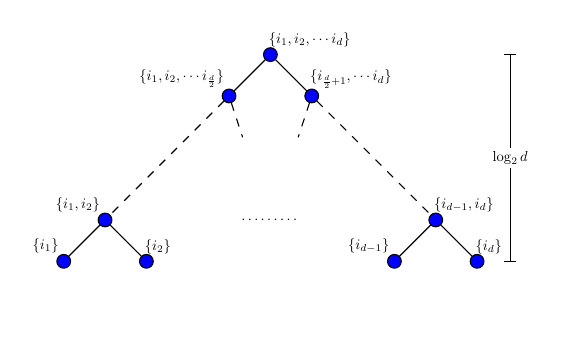
\begin{tikzpicture}[scale=0.525, every node/.style={transform shape}]
				
				\tikzstyle{taskc}=[circle, draw=black, minimum size=2mm, fill=blue]
				%%	\tikzstyle{taskr}=[draw=none, minimum height=2mm, minimum width=5mm, anchor=south west, fill=none, text=black]
				
				
				\node (t01) at (0,0) [taskc]{};
				\node (t11) at (-1,-1) [taskc] {};
				\node (t12) at (1, -1) [taskc] {};
				
				\node (tinter1) at (-0.5,-2) [taskc, draw=none, fill=none] {};
				\node (tinter2) at (0.5,-2) [taskc, draw=none, fill=none] {};
				
				\node (t41) at (-4,-4) [taskc] {};
				\node (t42) at (4,-4) [taskc] {};
				\node (t51) at (-5,-5) [taskc] {};
				\node (t52) at (-3,-5) [taskc] {};
				\node (t53) at (3,-5) [taskc] {};
				\node (t54) at (5,-5) [taskc] {};
				
				
				\draw (t01) -- (t11);
				\draw (t01) -- (t12);
				
				\draw [dashed] (t11) -- (tinter1.west);
				\draw [dashed] (t12) -- (tinter2.east);
				
				\draw [dashed] (t11) -- (t41);
				\draw [dashed] (t12) -- (t42);
				
				\path (t41) -- (t42) node [midway] {$\cdots\cdots\cdots$};
				
				\draw (t41) -- (t51);
				\draw (t41) -- (t52);
				
				\draw (t42) -- (t53);
				\draw (t42) -- (t54);
				
				
				\draw (5.8, -5) -- (5.8, -2.75);
				\draw (5.8, -2.25) -- (5.8, 0);
				
				\draw (5.65, -5) -- (5.95, -5);
				\draw (5.65, 0) -- (5.95, 0);
				\node at (5.8, -2.5) {$\log_2 d$};
				
				\node [above right] at (t01.160) {$\{i_1,i_2,\cdots i_d\}$};	
				
				\node [above left] at (t11.mid) {$\{i_1,i_2,\cdots i_\frac{d}{2}\}$};	
				\node [above right] at (t12.160) {$\{i_{\frac{d}{2}+1},\cdots i_d\}$};
				
				\node [above left] at (t41.mid) {$\{i_1,i_2\}$};
				\node [above right] at (t42.160) {$\{i_{d-1}, i_d\}$};
				
				\node [above left] at (t51.mid) {$\{i_1\}$};
				\node [above right] at (t52.160) {$\{i_2\}$};
				
				\node [above left] at (t53.mid) {$\{i_{d-1}\}$};
				\node [above right] at (t54.160) {$\{i_d\}$};
				
				
				\path (-0.1, -6.4) -- (2.5, -6.4); 
				%%		\path (-6.5, 0) -- (0,0);
				\end{tikzpicture}
			\end{center}
		\end{block}
	\end{minipage}
}\end{frame}


\begin{frame}{Parallelization of Density Matrix Renormalization Group (DMRG) algorithm}
\begin{center}
	\includegraphics[scale=0.275]{dmrg.png}\\
	\noindent (Fig source: Markus Reiher)$\qquad\qquad\qquad\qquad$\\
\end{center}


%%\medskip
\begin{block}{}
	\begin{itemize}
		\item Distribute load of $k$ number of sites on each node
		\item Perform computations in a tree structure
	\end{itemize}
\end{block}: 
\end{frame}

\end{document} 